\subsection{City Block Generation}

A city block in this project is defined as a continuous area of land which is suitable in shape, size, and position for containing multiple buildings.
The generation of such city blocks is managed by the BlockGenerator function (see Table~\ref{table:blockgen}).

\begin{table}[H]
  \centering
  \begin{tabular}{lllll}
    \textbf{Input}                           &               & \textbf{Function}            &               & \textbf{Output}         \\
    \midrule
    \textit{RoadNetwork, PopulationMap}      & $\rightarrow$ & \textbf{BlockGenerator}      & $\rightarrow$ & \textit{Block[]}        \\
    \bottomrule
  \end{tabular}

  \caption{Definition of the BlockGenerator function which is responsible for generating city blocks.}
  \label{table:blockgen}
\end{table}
\vspace{-0.4cm} % Mimic spacing below figures

% The example labels are incorrect, but I could make a code PR that fixes that.
This function uses the road network from the road generation to find suitable areas of land to extract, and it uses the population map from the population generation to determine which type of city block it should label each area as.
Examples of such labels include: \textit{industrial}, \textit{surburbs}, \textit{downtown}, \textit{skyscrapers}, \textit{appartments} and \textit{parks.}

The labeling of city blocks was implemented in a rather simple manner.
Each label was restricted to only occur within a specific range of population density and was given a weighted probability of occurring compared to other valid labels.
In practice, this was accomplished by assigning each label a probability distribution that could then be queried using the population density of the city block area.

The trickier part was to find suitable areas of land to extract into city blocks.
One approach composed of two iterations was considered, both of which treated the road network as an undirected graph.
The first iteration would find all the minimum cycles in the road network graph and extract the area enclosed by each cycle.
These areas would then be treated as city blocks if their size and shape seemed suitable.
A limitation of this iteration was that all blocks would be perfectly enclosed by roads.

The intention of the second iteration was to supplement the first by producing new cycles instead.
The idea was to traverse the outskirts of the graph and attempt to extend imaginary nodes.
These nodes would then help form new cycles as seen in Figure~\ref{fig:extend_block}.
The imaginary nodes would solely be used for defining the areas of the new city blocks, and would not contribute to the original road network.
This iteration would help counter the limitation mentioned in the first iteration, but unfortunately, only the first iteration was implemented due to time constraints.

% Drawn using https://csacademy.com/app/graph_editor/
% Since I only show my creation (and not their site) I don't need to cite.
\begin{figure}[h!]
  \centering
  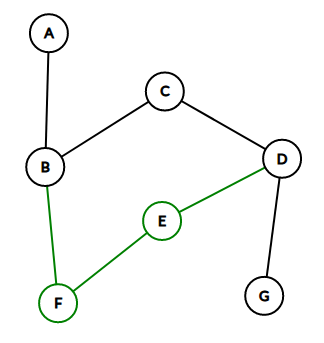
\includegraphics[width=0.35\textwidth]{figure/extend_block.png}

  \caption{Conceptual example of what the second city block extraction iteration could have produced. Here, the new cycle $BCDEF$ has been formed. Intersections are illustrated as nodes, roads as edges, and the extended block is colored green.}
  \label{fig:extend_block}
\end{figure}

The first iteration needed to find all minimum cycles in an undirected graph.
This is a known problem called Minimum Cycle Bases (MCB) and can be solved in $\mathcal{O}(m^3 + mn^2 \log n)$ or $\mathcal{O}(m^2n^2)$, for a graph with $n$ vertices and $m$ edges, using the efficient implementations proposed by Melhorn and Michail \cite{mcb_paper}.
These asymptotic time complexities might suffice for small cities, but not for multiple large ones.
Thus, either significant constraints had to be made, or another solution had to be found.

Fortunately, another solution was found.
Unlike typical graphs found in discrete mathematics, these road networks are constrained by a physical space, and are therefore a type of geometric graph.
Essentially, each node has a position relative to others and each edge has an angle relative to others.
With this information it actually becomes possible to solve the MCB problem, seemingly in only $\mathcal{O}(n + m)$.

The solution, first proposed by Petovan \cite{petovan}, can be described as follows:
\vspace{-0.5cm} % Reasonable spacing before list
\begin{enumerate}
  \item For each node, dispatch a \textit{turtle} along each connected edge.
  \item Let the \textit{turtle} traverse the graph by always following the edge closest (in counter-clockwise direction) to the previously traversed edge. Essentially, let the turtle always follow the rightmost edge relative to its current heading.
  \begin{enumerate}
    \item If the turtle tries to traverse some edge in a direction that has already been explored (potentially by another turtle), then terminate this turtle.
    \item If the turtle tries to traverse an edge it has already traversed, then terminate this turtle.
    \item If the turtle found back to the start node, then
      \begin{enumerate}
        \item if the turtle has turned an accumulated amount of 360 degrees conter-clockwise, discard it.
        \item otherwise, add the nodes the turtle visisted to a list of minimum cycles.
      \end{enumerate}
      %
  \end{enumerate}
  \item The resulting list of minimum cycles is the MCB of the graph.
\end{enumerate}

% Do we want to make a formal proof? Could be an appendix. Would be pretty cool to be first.
%The correctness nor runtime complexity of this algorithm has any known published proof, but an intution can still be gained.
Each turtle traverses the graph using the Pledge algorithm \cite{turtle_geometry}, which ensures that all non-terminated turtles will return to their start node.
The step \textit{2.a} ensures that all cycles have an area, and step \textit{2.c.i} handles the edge case where one turtle follows the perimeter of the whole graph.
The remaining cycles must be minimum since, otherwise, some edge would have to exist within the cycle but that edge would have been traversed by always following the rightmost edge, no matter the starting node (see Figure \ref{fig:graph_cycles}).
Thus, the correctness of the algorithm is shown.

% Drawn using https://csacademy.com/app/graph_editor/
\begin{figure}[h!]
  \centering
  \begin{subfigure}[b]{0.3\textwidth}
    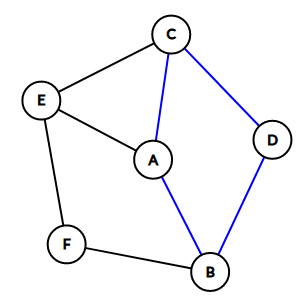
\includegraphics[width=\textwidth]{figure/blockgen1.png}
    %\caption{A minimum cycle.}
  \end{subfigure}
  \begin{subfigure}[b]{0.3\textwidth}
    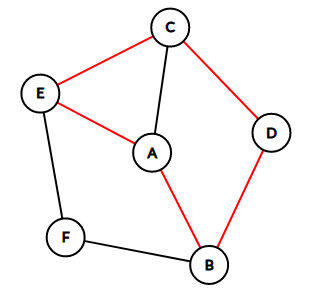
\includegraphics[width=\textwidth]{figure/blockgen2.png}
    %\caption{A non-minimum cycle.}
  \end{subfigure}

  \caption{Example of a minimum cycle (blue) and a non-minimum cycle (red). The red cycle has the edge \textit{AC} which splits the cycle into two minimum ones.}
  \label{fig:graph_cycles}
\end{figure}

Each edge is traversed twice (once from each direction) and each node is considered once for dispatching the turtles.
The rightmost edge can be queried in constant time by storing edges in counter-clockwise order in each node (and by storing array indices in the edges).
Thus, the algorithm runs in $\mathcal{O}(n + m)$.
With this efficiency, the generation of city blocks would no longer risk being a bottleneck.

Before returning, the BlockGenerator also insets the polygons of the resulting city blocks.
This step is needed to make sure the city blocks do not overlap with the road mesh of each edge.
Any further refinements of city blocks are subsequently handled by the plot generation.

